%!TEX root = ../dissertation.tex

\graphicspath{{4-methods/figures/}}
\chapter{Methods}
\label{ch:methods}

\section{Model Design}

\begin{figure}
	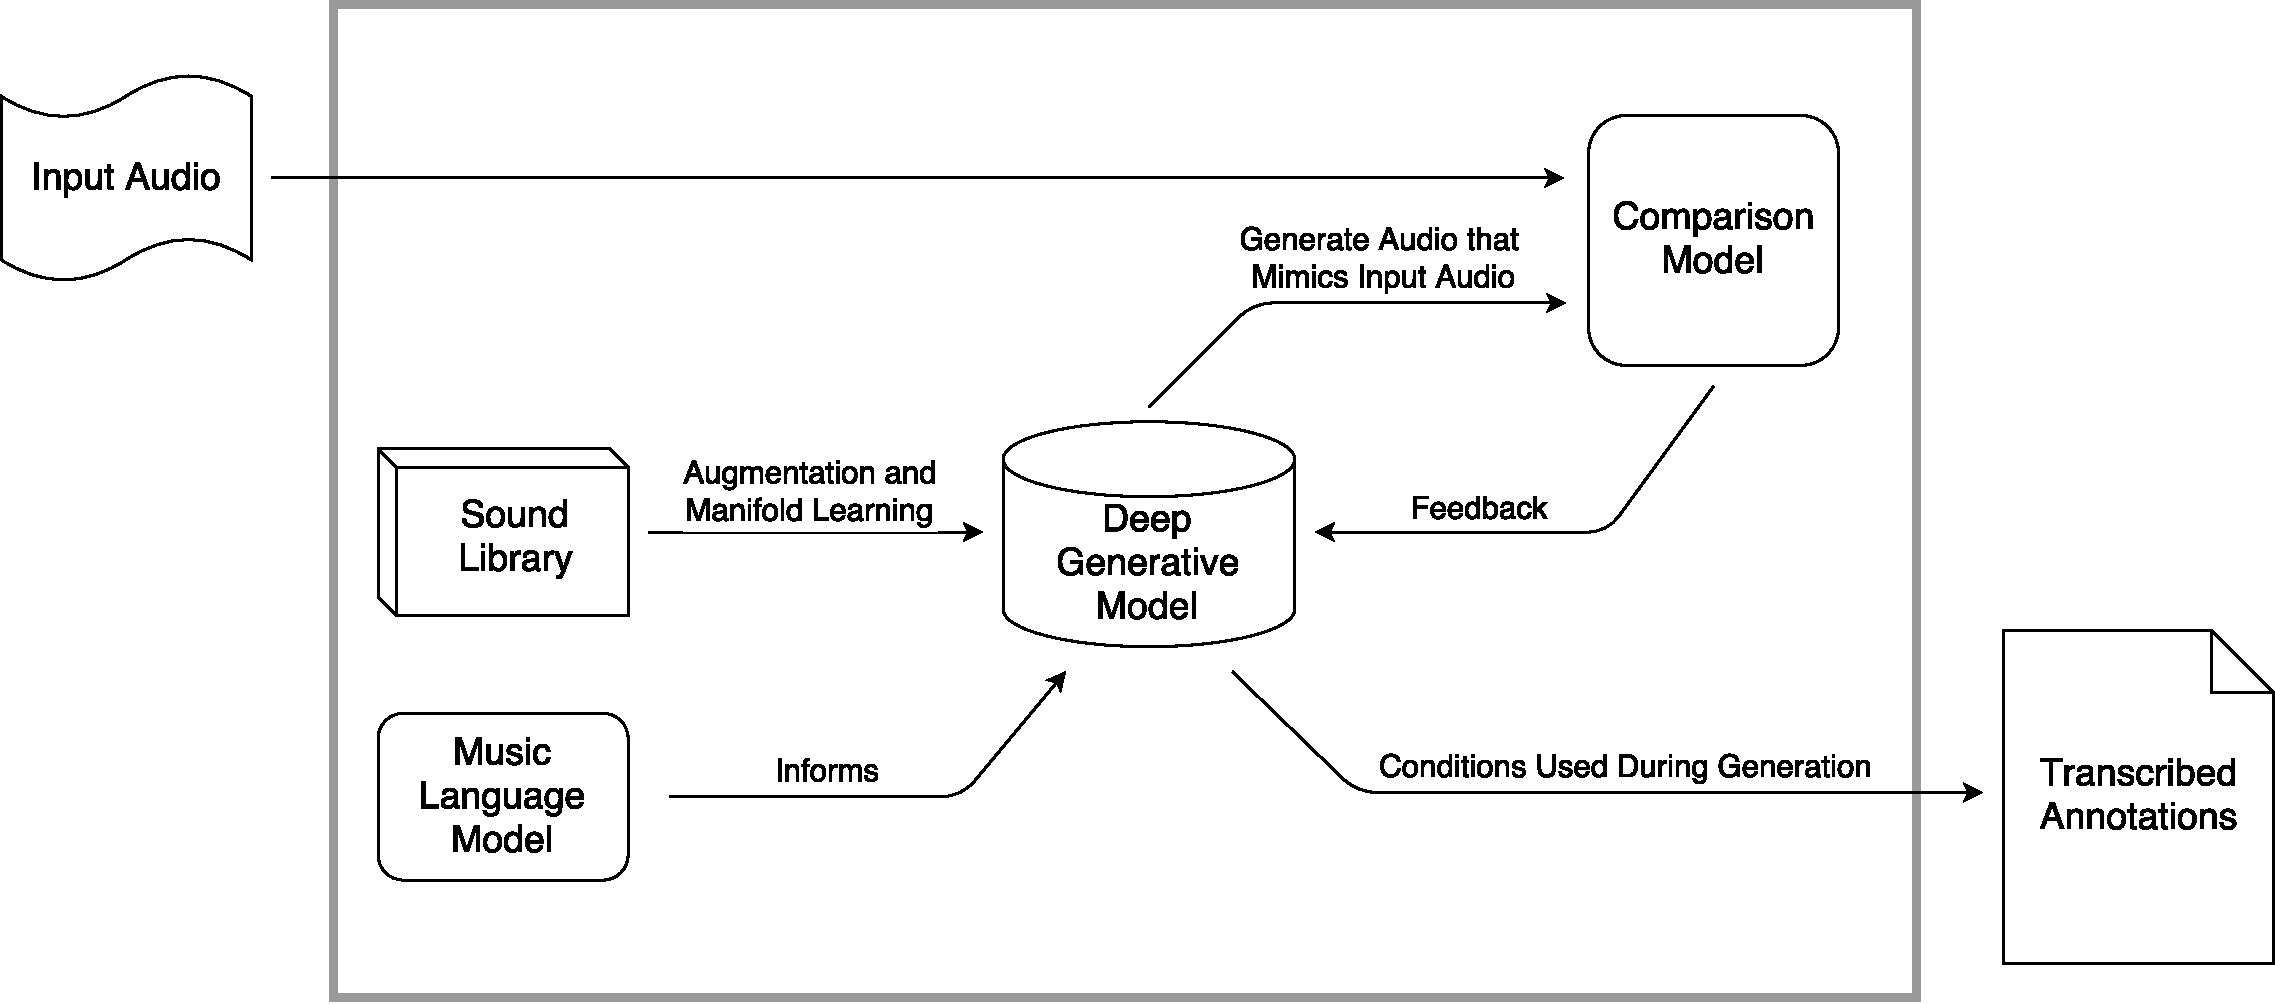
\includegraphics[width=\textwidth]{grand.pdf}
	\caption{The proposed architecture for the automatic music transcription pipeline. A deep generative model is trained using data augmentation and manifold learning on instrumental sound library, as well as a music language model, to generate audio track that sounds similarly as the input audio. The conditions used to generate the matching audio can produce the predicted music transcription.}\label{fig:grand}
\end{figure}

Figure \ref{fig:grand} shows the proposed architecture for an end-to-end automatic music transcription system.
In short, a deep generative model in the center will learn to generate audio signals that mimics the input, and the combinations of instruments and pitches used for generating that audio will be the resulting transcription.
The system is not only powered by deep generative models but also by a few other important techniques that will make the implementation possible to be realized.

Data augmentation is a method for increasing the quantity of available data using transformations that does not alter or deterministically alter the label, and has been successfully applied to image classification tasks  \cite{krizhevsky2012imagenet}. MUDA \cite{mcfee2015muda} provides a software framework for augmenting musical audio, which supports pitch shift, time stretch, background noise, and dynamic range compression.
One could also augment the data by filtering with the impulse responses according to various room acoustics, adding reverberations to the audio.
Combined with the audio sources from various software instruments and sample libraries, these methods for audio augmentation can greatly increase the amount of available training data, and will help the deep model to more accurately learn the distribution of the real-world musical sounds.

Synthesizing music is also an important part of the pipeline in Figure \ref{fig:grand}.
While sound synthesis is a topic that has a long history \cite{cook2002synthesis}, recent deep models were very successful in synthesizing breathtakingly high-quality audio signals.
WaveNet \cite{oord2016wavenet}, developed by Google DeepMind, uses a causal architecture using dilated convolutions to generate time-domain audio samples, and is able to produce realistic human voices and piano sounds.
There also exist faster approaches using recurrent neural networks to produce vocal and musical audio, as found in \cite{nayebi2015gruv} and \cite{kalingeri2016generation}, albeit with lower quality when compared to WaveNet.
Tacotron \cite{wang2017tacotron} is a fully end-to-end speech synthesizer that works directly on a sequence of characters, which can learn the pronunciation of unseen complex words and different ways of reading the same word according to the phrase semantics and punctuations.
SampleRNN \cite{mehri2016samplernn} formed a basis for the techniques used by Lyrebird, an AI startup founded by University of Montr\'{e}al students that provides API for synthesized voice of a specific person, e.g. Barack Obama.
A singing synthesis model \cite{blaauw2017singing} based on the WaveNet architecture is also capable of synthesizing voice parametrically, separating the influence of pitch and timbre in the model.
A music synthesis technique employing a similar approach as the above will be a key component of the overall architecture, allowing the transcription model to generate realistic-sounding music to compare with the input audio.

Lastly, another important component is the music language model that will help the music generator decide its parameters, i.e. the timbre and pitch.
Clearly, there is a similarity between music and human language \cite{patel2010musiclanguage}, and there have been approaches using recurrent neural network to build a music language models \cite{sigtia2014lm}.
There are decades-long history of algorithmic composition techniques \cite{fernandez2013ai}, where MidiNet \cite{yang2017midinet} is the one of the latest example which generates symbolic music using a generative adversarial network.

\section{Datasets}

The experiments are based on a few publicly and commercially available datasets including RWC Music Database \cite{goto2003rwc}, MedleyDB \cite{bittner2014medleydb}, and Vienna Symphonic Library of orchestral sounds as studied in \cite{humphrey2011nlse}.
In future studies, the NSynth Dataset published recently by Google's Magenta project \cite{engel2017nsynth} is also planned to be used, as the dataset contains additional kinds of instruments and comes with more accurate annotations.


